%! alt Triangle ABC in its circumcircle with centre O. On BC lie the midpoint E, the foot D of the bisector from A, and, beyond C, the foot F of the altitude from A, with DE = 3, DF = 12 and AF = 16. The bisector AD is extended to N, the lowest point of the circle, directly below E with NE = 4. The shaded right triangles DEN and DFA are similar, and dashed segments join O to N and to B.
%! after_paragraph 1
%! scale 1/6
%! let R = 125/8
% The shared preamble of every Cevian figure. pipeline/figures turns these colours into theme-aware paint,
% and refuses any other colour, so draw only with them:
%   figink (lines and labels), figaux (construction lines), figaccent (the object the argument turns on),
%   figtint and figaccenttint (light fills).
\documentclass[border=1.5pt]{standalone}
\usepackage{tkz-euclide}
\definecolor{figink}{RGB}{0,0,0}
\definecolor{figaux}{RGB}{85,85,85}
\definecolor{figaccent}{RGB}{192,57,43}
\definecolor{figtint}{RGB}{221,221,221}
\definecolor{figaccenttint}{RGB}{245,213,208}
% tkz-euclide's defaults draw circles, compasses and marks in 50% grey and fill points with a tint.
\makeatletter
\def\tkz@otherlinecolor{figink}
\def\tkz@euc@circlecolor{figink}
\def\tkz@euc@compasscolor{figink}
\def\tkz@euc@mkcolor{figink}
\def\tkz@mk@fill{figink}
\def\tkz@euc@pointfillcolor{figink}
\makeatother
\tkzSetUpLine[color=figink,line width=.7pt]
\tkzSetUpArc[color=figink,line width=.7pt]
\tkzSetUpCompass[color=figink,line width=.5pt]
\tkzSetUpPoint[color=figink,fill=figink,size=3.1pt]
\tikzset{
  every picture/.style={line cap=round,line join=round,color=figink},
  circle style/.append style={color=figink,line width=.7pt},
  aux/.style={color=figaux,line width=.45pt,dash pattern=on 2.6pt off 2pt},
  key/.style={color=figaccent,line width=1pt},
  mk/.style={color=figink,line width=.5pt},
  lbl/.style={color=figink,inner sep=2.2pt},
  len/.style={color=figink,inner sep=1.5pt,font=\small},
}

\begin{document}
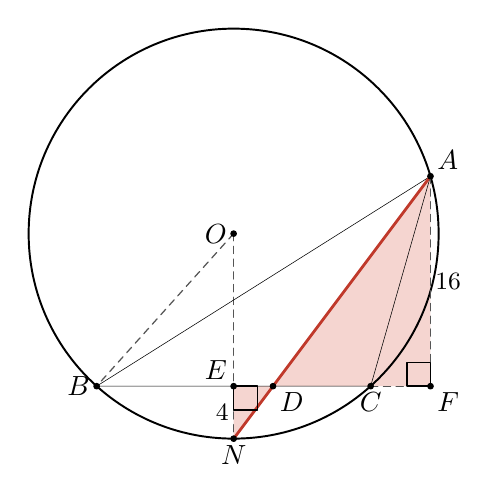
\begin{tikzpicture}
\tkzDefPoint(0.0,0.0){E} %! E = (0, 0)
\tkzDefPoint(0.50000000,0.0){D} %! D = (3, 0)
\tkzDefPoint(2.5000000,0.0){F} %! F = (15, 0)
\tkzDefPoint(2.5000000,2.6666667){A} %! A = (15, 16)
\tkzDefPoint(-1.7400511,0.0){B} %! B = (-sqrt(109), 0)
\tkzDefPoint(1.7400511,0.0){C} %! C = (sqrt(109), 0)
\tkzDefPoint(0.0,-0.66666667){N} %! N = (0, -4)
\tkzDefPoint(0.0,1.9375000){O} %! O = (0, 93/8)
%! fact dist(D, E) == 3
%! fact dist(D, F) == 12
%! fact dist(A, F) == 16
%! fact perp(A, F, B, C)
%! fact midpoint(E, B, C)
%! fact on_segment(D, B, C)
%! fact equal(angle(B, A, D), angle(D, A, C))
%! fact collinear(N, A, D)
%! fact on_circle(A, O, R)
%! fact on_circle(B, O, R)
%! fact on_circle(C, O, R)
%! fact on_circle(N, O, R)
%! fact perp(N, E, B, C)
%! fact dist(N, E) == 4
%! fact dist(D, N) == 5
%! fact dist(A, D) == 20
%! fact dist(D, B)*dist(D, C) == 100
%! fact dist(E, B)**2 == 109
%! fact dist(O, A) == 125/8
\tkzFillPolygon[color=figaccenttint](D,E,N)
\tkzFillPolygon[color=figaccenttint](D,F,A)
\tkzDrawCircle(O,A)
\tkzDrawSegment[aux](C,F)
\tkzDrawSegment[aux](A,F)
\tkzDrawSegment[aux](O,N)
\tkzDrawSegment[aux](O,B)
\tkzDrawPolygon(A,B,C)
\tkzDrawSegment[key](A,N)
\tkzMarkRightAngle[size=.3,mk](A,F,D)
\tkzMarkRightAngle[size=.3,mk](N,E,D)
\tkzDrawPoints(A,B,C,D,E,F,N,O)
\tkzLabelPoint[above right,lbl](A){$A$}
\tkzLabelPoint[left,lbl](B){$B$}
\tkzLabelPoint[below,lbl](C){$C$}
\tkzLabelPoint[below right,lbl](D){$D$}
\tkzLabelPoint[above left,lbl](E){$E$}
\tkzLabelPoint[below right,lbl](F){$F$}
\tkzLabelPoint[below,lbl](N){$N$}
\tkzLabelPoint[left,lbl](O){$O$}
\tkzLabelSegment[right,len](A,F){$16$}
\tkzLabelSegment[left,len](E,N){$4$}
\end{tikzpicture}
\end{document}
